\documentclass[polish, 8pt]{article}
\usepackage[top=2cm, bottom=2cm, left=3cm, right=3cm]{geometry}
\usepackage{graphicx} % Required for inserting images

\usepackage[polish]{babel}
\usepackage{polski}
\usepackage{placeins}
\usepackage{dirtytalk}
% Set page size and margins
% Replace `letterpaper' with `a4paper' for UK/EU standard size
\usepackage{csquotes}
% Useful packages
\usepackage{float}
\usepackage{amsmath}
\usepackage{graphicx}
\usepackage{hyperref}
\usepackage{graphicx}
\usepackage{listings}
\usepackage{xcolor}
\usepackage{amssymb}
\usepackage{enumitem}
\usepackage{float}
\definecolor{codegreen}{rgb}{0,0.6,0}
\definecolor{codegray}{rgb}{0.5,0.5,0.5}
\definecolor{codepurple}{rgb}{0.58,0,0.82}
\definecolor{backcolour}{rgb}{0.95,0.95,0.92}
\usepackage{amsmath, amssymb, tikz}
\lstdefinestyle{mystyle}{
    backgroundcolor=\color{backcolour},   
    commentstyle=\color{codegreen},
    keywordstyle=\color{magenta},
    numberstyle=\tiny\color{codegray},
    stringstyle=\color{codepurple},
    basicstyle=\ttfamily\footnotesize,
    breakatwhitespace=false,         
    breaklines=true,                 
    captionpos=b,                    
    keepspaces=true,                 
    numbers=left,                    
    numbersep=5pt,                  
    showspaces=false,                
    showstringspaces=false,
    showtabs=false,                  
    tabsize=2
}
\lstset{style=mystyle}
\hypersetup{
    colorlinks=true,
    linktoc=all     %set to all if you want both sections and subsections linked
}

\title{Rachunek Prawdopodobieństwa i Statystyka -- Kolokwium I}
\author{}
\date{}


\begin{document}
\maketitle

\section*{Zadanie 1}
Wizualizujemy sytuację przy pomocy drzewka:

\begin{figure}[H]
    \centering
    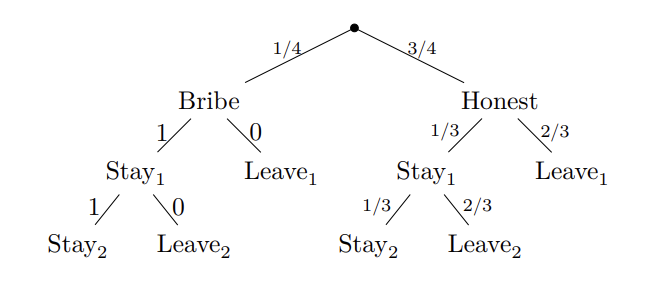
\includegraphics[width=300pt]{tree.png}
\end{figure}

Wprowadzamy następujące oznaczenia:
\begin{itemize}
    \item \( B \): uczestnik przekupuje sędziów,
    \item \( H \): uczestnik jest uczciwy (nie przekupuje sędziów),
    \item \( S_1 \): uczestnik został w pierwszym odcinku,
    \item \( S_2 \): uczestnik został w drugim odcinku,
    \item \( L_1 \): uczestnik został wyrzucony w pierwszym odcinku,
    \item \( L_2 \): uczestnik został wyrzucony w drugim odcinku.
\end{itemize}

\subsection*{a)}

Najpierw obliczamy \( P(S_1) \) korzystając z tw. o prawdopodobieństwie całkowitym:
\[
P(S_1) = P(S_1|B)P(B) + P(S_1|H)P(H)
\]
\[
P(S_1) = 1 \cdot \frac{1}{4} + \frac{1}{3} \cdot \frac{3}{4} = \frac{1}{4} + \frac{1}{4} = \frac{1}{2}.
\]
Następnie obliczamy $P(B|S_1)$ z twierdzenia Bayesa:
\[
P(B|S_1) = \frac{P(S_1|B)P(B)}{P(S_1)} = \frac{1 \cdot \frac{1}{4}}{\frac{1}{2}} = \frac{1}{2}.
\]

\subsection*{b)}

Korzystając z drzewka, możemy obliczyć prawdopodobieństwo \( S_2 \):
\[
P(S_2) = P(S_2 | S1, B) P(S1 | B) P(B) + P(S_2 | S1, H) P(S1 | H) P(H) = 1 \cdot 1 \cdot \frac{1}{4} + \frac{1}{3} \cdot \frac{1}{3} \cdot \frac{3}{4} = \frac{1}{3}.
\]

\subsection*{c)}

Chcemy obliczyć \( P(L_2 | S_1) \):
\[
P(L_2 | S_1) = \frac{P(L_2 \cap S_1)}{P(S_1)}.
\]
Z poprzednich obliczeń mamy \( P(S_1) = \frac{1}{2} \). Dla licznika, korzystając z drzewka:
\[
P(L_2 \cap S_1) = P(L_2 \cap S_1 | B)P(B) + P(L_2 \cap S_1 | H)P(H).
\]
\[
P(L_2 \cap S_1) = 0 \cdot 1 \cdot \frac{1}{4} + \frac{2}{3} \cdot \frac{1}{3} \cdot \frac{3}{4} = \frac{1}{6}.
\]
Zatem:
\[
P(L_2 | S_1) = \frac{\frac{1}{6}}{\frac{1}{2}} = \frac{1}{3}.
\]
\section*{Zadanie 2}
Nasza teza:
\[
P(A, B) \geq P(A) + P(B) - 1,
\]
jest równoważna:
\[
1 \geq P(A) + P(B) - P(A, B).
\]
\subsection*{Krok 1: Przekształcenie nierówności}
Korzystamy z własności:
\[
P(A) + P(B) - P(A, B) = P(A \cup B).
\]
Z powyższego wynika, że teza jest równoważna nierówności:
\[
1 \geq P(A \cup B).
\]
\subsection*{Krok 2: Własność prawdopodobieństwa}
Wiemy, że dla dowolnego zdarzenia \( C \in \Sigma \) zachodzi:
\[
1 \geq P(C),
\]
co implikuje, że:
\[
1 \geq P(A \cup B),
\]
i tym samym kończy dowód.

\section*{Zadanie 3}

Dla funkcji gęstości prawdopodobieństwa:
\[
f(x) =
\begin{cases}
ax + bx^2 & \text{dla } 0 \leq x \leq 1, \\
0 & \text{w przeciwnym przypadku.}
\end{cases}
\]

\subsection*{Krok 1: Warunek}
Funkcja gęstości prawdopodobieństwa musi spełniać następujący warunek:
\[
\int_{-\infty}^\infty f(x) \, dx = 1.
\]
W naszym przypadku:
\[
\int_{-\infty}^\infty f(x) \, dx = \int_{-\infty}^0 0 \, dx +  \int_0^1 (ax + bx^2) \, dx + \int_{1}^\infty 0 \, dx = 1.
\]
Obliczamy całkę:
\[
\int_{-\infty}^\infty f(x) \, dx = \int_0^1 (ax + bx^2) \, dx = \int_0^1 ax \, dx + \int_0^1 bx^2 \, dx = \left[\frac{a x^2}{2}\right]_0^1 + \left[\frac{b x^3}{3}\right]_0^1 = \frac{a}{2} + \frac{b}{3}.
\]
Ostatecznie dostajemy:
\[
\frac{a}{2} + \frac{b}{3} = 1. \tag{1}
\]

\subsection*{Krok 2: Wartość oczekiwana}
Wartość oczekiwana zmiennej losowej \(X\) wynosi:
\[
\mathbb{E}(X) = \int_{-\infty}^\infty x f(x) \, dx.
\]
Analogicznie wystarczy, że skupimy się na przedziale \(0 \leq x \leq 1\):
\[
\mathbb{E}(X) = \int_0^1 x(ax + bx^2) \, dx = \int_0^1 (ax^2 + bx^3) \, dx.
\]
Obliczamy całkę:
\[
\int_0^1 (ax^2 + bx^3) \, dx = \int_0^1 ax^2 \, dx + \int_0^1 bx^3 \, dx = \left[\frac{a x^3}{3}\right]_0^1 + \left[\frac{b x^4}{4}\right]_0^1 = \frac{a}{3} + \frac{b}{4}.
\]
Z warunku:
\[
\mathbb{E}(X) = \frac{7}{12},
\]
otrzymujemy:
\[
\frac{a}{3} + \frac{b}{4} = \frac{7}{12}. \tag{2}
\]

\subsection*{Krok 3: Rozwiązanie układu równań}
Rozwiązujemy układ równań:
\[
\begin{cases} 
\frac{a}{2} + \frac{b}{3} = 1, \\ 
\frac{a}{3} + \frac{b}{4} = \frac{7}{12}.
\end{cases}
\]
Mnożymy pierwsze równanie przez 18, drugie równanie przez 24:
\[
\begin{cases} 
9a + 6b = 18, \\ 
8a + 6b = 14.
\end{cases}
\]
Odejmujemy równania stronami i otrzymujemy:
\[
\begin{cases} 
a = 4, \\ 
b = \frac{18 - 9a}{6} = -3.
\end{cases}
\]

\subsection*{Krok 4: Wariancja}
Wariancja \(Var(X)\) jest dana wzorem:
\[
Var(X) = \mathbb{E}(X^2) - (\mathbb{E}(X))^2.
\]
Obliczamy \(\mathbb{E}(X^2)\) (znowu ograniczamy się do przedziału \(0 \leq x \leq 1\)):
\[
\mathbb{E}(X^2) = \int_0^1 x^2 f(x) \, dx = \int_0^1 x^2(4x - 3x^2) \, dx = \int_0^1 (4x^3 - 3x^4) \, dx.
\]
\[
\int_0^1 (4x^3 - 3x^4) \, dx = \left[x^4 - \frac{3x^5}{5}\right]_0^1 = 1 - \frac{3}{5} = \frac{2}{5}.
\]
Zatem:
\[
Var(X) = \frac{2}{5} - \left(\frac{7}{12}\right)^2 = \frac{2}{5} - \frac{49}{144}.
\]
Po sprowadzeniu do wspólnego mianownika:
\[
Var(X) = \frac{288}{720} - \frac{245}{720} = \frac{43}{720}.
\]
\subsection*{Krok 5: Moda}
Moda to wartość \(x\), dla której \(f(x)\) osiąga maksimum. Pochodna \(f(x)\) wynosi:
\[
f'(x) = 4 - 6x.
\]
Zatem \(f'(x) = 0\) dla \(x = \frac{2}{3}\). Sprawdzamy znak pochodnej i potwierdzamy, że maksimum występuje w \(x = \frac{2}{3}\). W tym podpunkcie można również zauważyć, że $f(x)$ jest funkcją kwadratową i obliczyć pierwszą współrzędną wierzchołka.

\subsection*{Krok 6: Wyznaczenie dystrybuanty \(F_X(x)\)}
Dystrybuanta \(F_X(x)\) jest dana wzorem:
\[
F_X(x) = \int_{-\infty}^x f(t) \, dt.
\]
Dla \(x \in [0, 1]\):
\[
F_X(x) = \int_0^x (4t - 3t^2) \, dt = \left[2t^2 - t^3\right]_0^x = 2x^2 - x^3.
\]
Dla \(x < 0\), \(F_X(x) = 0\), a dla \(x > 1\), \(F_X(x) = 1\). Ostatecznie:
\[
F_X(x) =
\begin{cases}
0 & \text{dla } x < 0, \\
2x^2 - x^3 & \text{dla } 0 \leq x \leq 1, \\
1 & \text{dla } x > 1.
\end{cases}
\]

\subsection*{Krok 7: Obliczenie \(P(|X| < \frac{1}{2})\)}
\[
P(|X| < \frac{1}{2}) = P\left(-\frac{1}{2} < X < \frac{1}{2}\right).
\]
Ponieważ \(P(X < 0) = 0\), mamy:
\[
P(|X| < \frac{1}{2}) = P\left(0 < X < \frac{1}{2}\right).
\]
Obliczamy:
\[
P\left(0 < X < \frac{1}{2}\right) = F_X\left(\frac{1}{2}\right) - F_X(0).
\]
Dla \(x = \frac{1}{2}\):
\[
F_X\left(\frac{1}{2}\right) = 2\left(\frac{1}{2}\right)^2 - \left(\frac{1}{2}\right)^3 = 2 \cdot \frac{1}{4} - \frac{1}{8} = \frac{1}{2} - \frac{1}{8} = \frac{4}{8} - \frac{1}{8} = \frac{3}{8}.
\]
Dla \(x = 0\), \(F_X(0) = 0\). Ostatecznie:
\[
P(|X| < \frac{1}{2}) = \frac{3}{8} - 0 = \frac{3}{8}.
\]

\section*{Zadanie 4}

Oba lotniska są takie same, lądowanie samolotów jest niezależne w związku z tym skupiamy się na jednym lotnisku. Niech \( t_A \) i \( t_B \) będą czasami rozpoczęcia lądowania odpowiednio dla samolotów A i B, równomiernie rozłożonymi na \([0, 30]\). W związku z tym:
\[
\Omega = \{(t_A, t_B): (t_A, t_B) \in [0, 30]^2 \}
\]
Od razu zauważamy, że:
\[
|\Omega| = 30 \cdot 30 = 900.
\]
Brak czekania samolotów występuje, gdy:
\[
t_A \leq t_B \land t_A + 7 \leq t_B \quad \text{lub} \quad t_B \leq t_A \land t_B + 9 \leq t_A.
\]
Przy pomocy $A$ oznaczamy zdarzenie lądowania pary samolotów bez czekania.
\[
A = \{(t_A, t_B) \in \Omega, t_A + 7 \leq t_B \land t_B + 9 \leq t_A \}
\]
$\Omega$ to kwadrat $[0,30]^2$, $A$ to część kwadratu wyznaczana przez proste $t_A + 7 \leq t_B$ i $t_B + 9 \leq t_A$.
\begin{figure}[H]
    \centering
    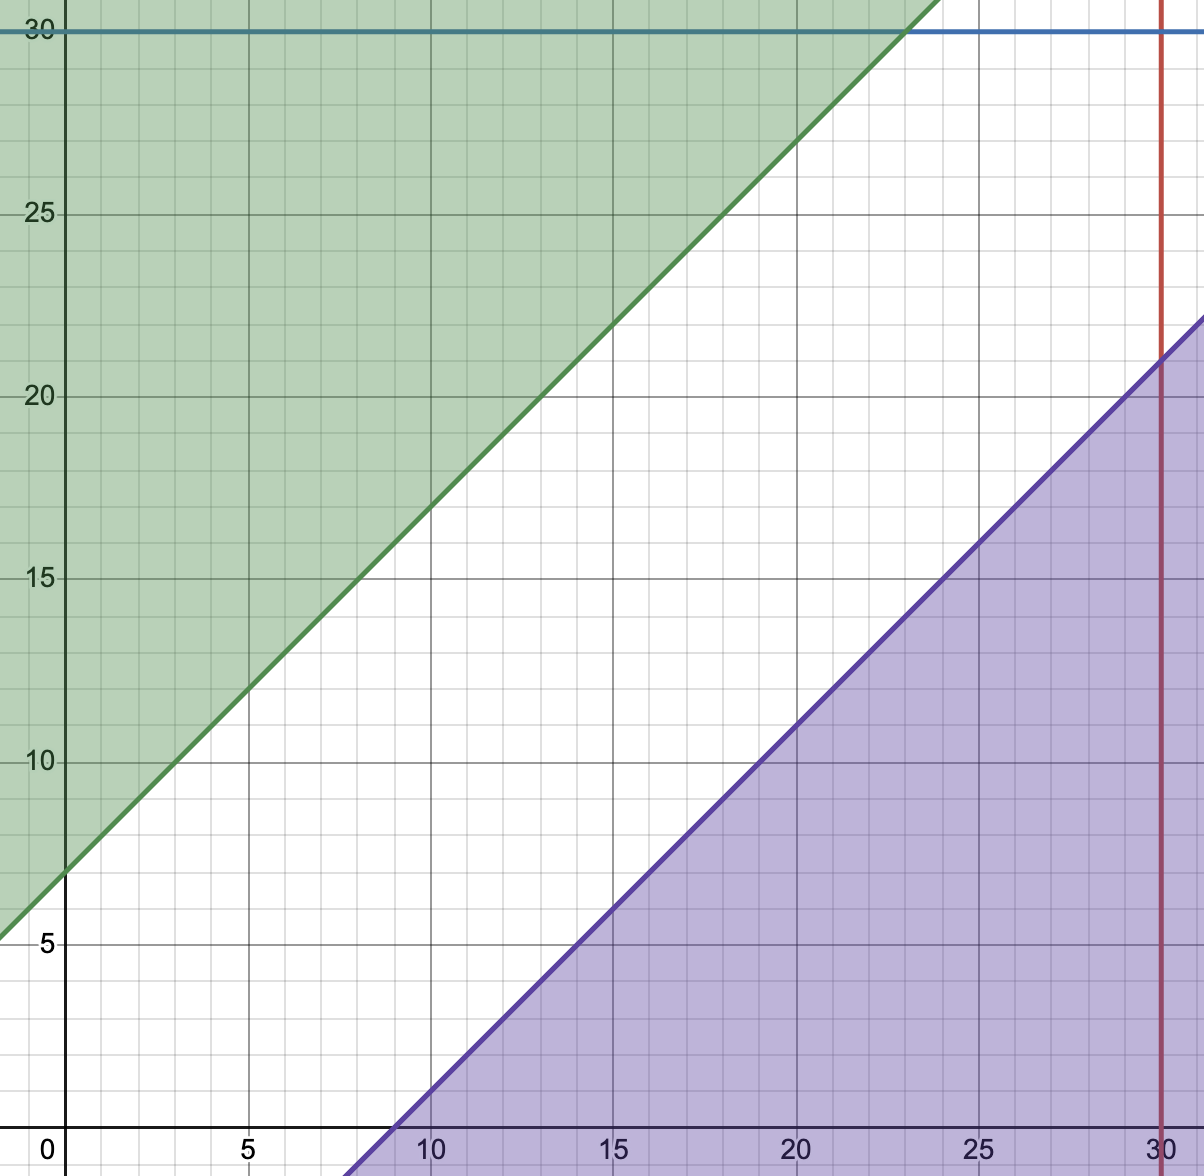
\includegraphics[width=300pt]{flight.png}
    \caption{Wizualizacja $A$}
\end{figure}
Możemy zauważyć, że $A$ składa się z dwóch trójkątów prostokątnych, równoramiennych. Zielony trójkąt ma przyprostokątne długości $30 - 7 = 23$, fioletowy ma przyprostokątne długości $30 - 9 = 21$. W związku z tym:
\[
|A| = |\Delta_{Z}| + |\Delta_{F}| = \frac{23^2}{2} + \frac{21^2}{2} = \frac{529}{2} + \frac{441}{2} = \frac{970}{2} = 485.
\]
Obliczamy $P(A)$:
\[
P(A) = \frac{|A|}{|\Omega|} = \frac{485}{900} = \frac{97}{180}
\]
Wiemy, że są dwa lotniska. Niech $B$ oznacza, że przynajmniej na jednym
z lotnisk samoloty nie będą na siebie czekać. Zdarzenie przeciwne do $B$ to sytuacja, w której samoloty czekają na siebie na obu lotniskach:
\[
P(B') = 1 - P(B) = P(A_1', A_2') 
\]
Korzystamy z tego, że lotniska są takie same:
\[
P(A_1) = P(A_2) = P(A) \implies P(A_1') = P(A_2') = 1 - P(A)
\]
i z niezależności lądowań:
\[
P(B') = 1 - P(B) = P(A_1', A_2') = P(A_1') P(A_2') = (1-P(A))^2
\]
Wynika z tego, że:
\[
P(B) = 1 - (1 - P(A))^2 = 1 - \bigl(1 - \frac{97}{180}\big)^2 = 1 - \bigl(\frac{83}{180}\big)^2
\]


\section*{Zadanie 5}

\subsection*{Krok 1: Rozkład zmiennej \( X \)}
Zmienna \( X \) ma rozkład jednostajny na przedziale \( [a, b] \), gdzie \( 0 < a < b \). Funkcja gęstości prawdopodobieństwa \( f_X(x) \) wynosi:
\[
f_X(x) =
\begin{cases}
\frac{1}{b-a}, & \text{dla } x \in [a, b], \\
0, & \text{w przeciwnym przypadku}.
\end{cases}
\]
Dystrybuanta \( F_X(x) \) jest zdefiniowana jako:
\[
F_X(x) =
\begin{cases}
0, & \text{dla } x < a, \\
\frac{x-a}{b-a}, & \text{dla } x \in [a, b], \\
1, & \text{dla } x > b.
\end{cases}
\]

\subsection*{Krok 2: Wyznaczenie rozkładu zmiennej \( Y = \ln(X) \)}
Zmienna \( Y \) jest zdefiniowana jako \( Y = \ln(X) \), więc \( X = e^Y \). Korzystamy z metody dystrybuanty:
\[
F_Y(y) = P(Y \leq y) = P(lnX \leq y) = P(X \leq e^y) = F_X(e^y)
\]
Różniczkujemy obustronnie i otrzymujemy:
\[
f_Y(y) = F_Y'(y) = f_X(e^y) \cdot (e^y)' = f_X(e^y) \cdot e^y.
\]
Ostatecznie, funkcja gęstości \( f_Y(y) \) wynosi:
\[
f_Y(y) =
\begin{cases}
\frac{e^y}{b-a}, & \text{dla } y \in [\ln(a), \ln(b)], \\
0, & \text{w przeciwnym razie}.
\end{cases}
\]
Warto zwrócić uwagę na przedział $[\ln(a), \ln(b)]$. W przypadku $X$: $f_X(x) \neq 0$ dla $x \in [a, b]$. Wiemy, że $f_Y(y) = f_X(e^y) \neq 0$ dla $e^y \in [a, b]$, co daje $y \in [ln(a), ln(b)]$.\\
Wyznaczamy dystrybuantę \( F_Y(y) \):
\[
F_Y(y) =
\begin{cases}
0, & \text{dla } y < \ln(a), \\
\frac{e^y - a}{b-a}, & \text{dla } y \in [\ln(a), \ln(b)], \\
1, & \text{dla } y > \ln(b).
\end{cases}
\]
\subsection*{Krok 3: Wyrażenie \( P(c < Y \leq d) \)}
Prawdopodobieństwo \( P(c < Y \leq d) \) obliczamy przy pomocy dystrybuanty:
\[
P(c < Y \leq d) = F_Y(d) - F_Y(c).
\]
Szukamy $c, d$ takich że:
\[
P(c < Y \leq d) = F_Y(d) - F_Y(c) = f_Y(d) - f_Y(c)
\]
Rozważamy wszystkie przypadki:
\subsubsection*{Przypadek I: \( c,d < \ln(a) \)}
\[
 F_Y(d) - F_Y(c) = 0 - 0 = 0 - 0 = f_Y(d) - f_Y(c)
\]
Równość zachodzi.

\subsubsection*{Przypadek II: \( c < \ln(a), d \in [\ln(a), \ln(b)] \)}
\[
 F_Y(d) - F_Y(c) = \frac{e^d - a}{b-a} - 0 \neq \frac{e^d}{b-a} - 0 = f_Y(d) - f_Y(c)
\]
Równość nie zachodzi o ile $a \neq 0$.

\subsubsection*{Przypadek III: \( c < \ln(a), d > \ln(b) \)}
\[
 F_Y(d) - F_Y(c) = 1 - 0 \neq 0 - 0 = f_Y(d) - f_Y(c)
\]
Równość nie zachodzi.

\subsubsection*{Przypadek IV: \( c,d \in [\ln(a), \ln(b)] \)}
\[
 F_Y(d) - F_Y(c) = \frac{e^d - a}{b-a} - \frac{e^c - a}{b-a} = \frac{e^d}{b-a} - \frac{e^c}{b-a} = f_Y(d) - f_Y(c)
\]
Równość zachodzi.

\subsubsection*{Przypadek V: \( c \in [\ln(a), \ln(b)], d > \ln(b) \)}
\[
 F_Y(d) - F_Y(c) = 1 - \frac{e^c - a}{b-a} \neq 0 - \frac{e^c}{b-a} = f_Y(d) - f_Y(c)
\]
Równość nie zachodzi, ponieważ prawa strona jest ujemna.

\subsubsection*{Przypadek VI: \( c, d > \ln(b) \)}
\[
 F_Y(d) - F_Y(c) = 1 - 1 = 0 - 0 = f_Y(d) - f_Y(c)
\]
Równość zachodzi.

\end{document}

